\documentclass[12pt]{beamer}
\usetheme{CambridgeUS}
\usecolortheme{dolphin}

\usepackage[utf8]{inputenc}
\usepackage[brazil]{babel}
\usepackage[T1]{fontenc}
\usepackage{xcolor}
\usepackage{amsmath}
\usepackage{amsfonts}
\usepackage{amssymb}
\usepackage{graphicx}
\usepackage{setspace}
\usepackage{ragged2e}

\setbeamertemplate{caption}[numbered]

% Controle do gabarito %
%%%%%%%%%%%%%%%%%%%%%
\newif\ifgab
\gabtrue
\newcommand{\gab}[1]{%
  \ifgab
    \textcolor{red!80!black}{\textbf{#1}}%
  \else
    #1%
  \fi
}
%%%%%%%%%%%%%%%%%%%%%

\author[Joao Victor]{Pibidiano: Joao Victor}
\title[Estágio Supervisionado I]{Estágio Supervisionado I \\ Ensino Fundamental II}
%\setbeamercovered{transparent} 
\setbeamertemplate{navigation symbols}{} 
\institute[]{CETi BILÍNGUE GILBERTO MESTRINHO} 
\date{\today} 
\titlegraphic{
\includegraphics[width=0.25\textwidth]{imagens/estagio.png}}

%\subject{}

% ---------------------------------------------------------

\begin{document}
\justifying
\onehalfspacing 

\begin{frame}
    \titlepage
\end{frame}

\section{Dados Gerais}

	\begin{frame}{Dados Gerais}
		\begin{itemize}
			\justifying
			\item EETI Gilberto Mestrinho de Medeiros Raposo;
			\item Localizada no bairro Educandos (zona sul de Manaus);
			\item Turmas: Do 6º ao 9º ano; e Ensino Médio;
			\item Espaço Maker: é o 51º a ser entregue pelo Governo do Amazonas, de um total de 100.
		\end{itemize}
	\end{frame}
	
\section{PIBID - Parte I}
	
	\begin{frame}{Turmas: 7º e 8º anos}
		\begin{itemize}
			\justifying
			\item Professora supervisora: Nalva Cristina;
			\item Estudei com a filha dela: Carlla Vicna dos Reis Martins;
			\item Projetos Extensionistas e treino de tabuada;
			\item Respeito instantâneo dos alunos em sala;
			\item Co-autora em trabalhos que levei para a Semana da Matemática (UEA - 2025) e Encontro Nacional das Licenciaturas (ENALIC).
		\end{itemize}
	\end{frame}
	
	\begin{frame}{PIBID - Parte I}
		\centering
		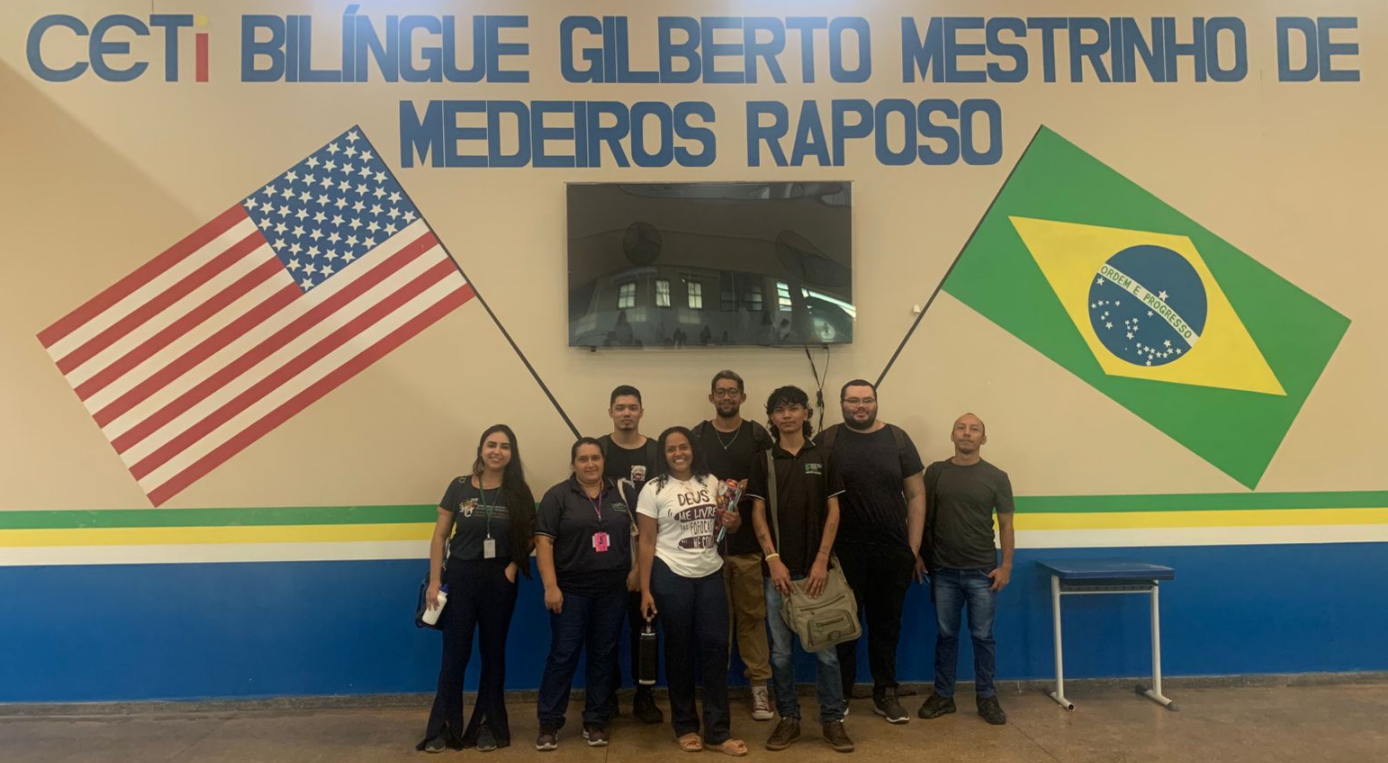
\includegraphics[scale=0.25]{imagens/nalva2.png}
	\end{frame}
\section{PIBID - PARTE II}

	\begin{frame}{Turmas: 7º, 8º e 9º anos}
		\begin{itemize}
			\justifying
			\item Supervisor: Prof. Elioney Pereira;
			\item Aulas com uso Power Point; IA's; Práticas;
			\item Fomento à Gincana de Matemática;
			\item Elaboração de Provas (criativas);
			\item Co-autor em trabalhos submetidos na Semana de Matemática (UEA - 2026), Encontro das Licenciaturas da Região Norte - I Enlic Norte (UEA - 2026) e ao Simpósio da Associação Latino-americana de Investigação em Educação em Ciências - LASERA (UEA - 2026)
		\end{itemize}
	\end{frame}
	
\section{Destaques da Escola}

	\begin{frame}{Gincana de Matemática}
		\centering
		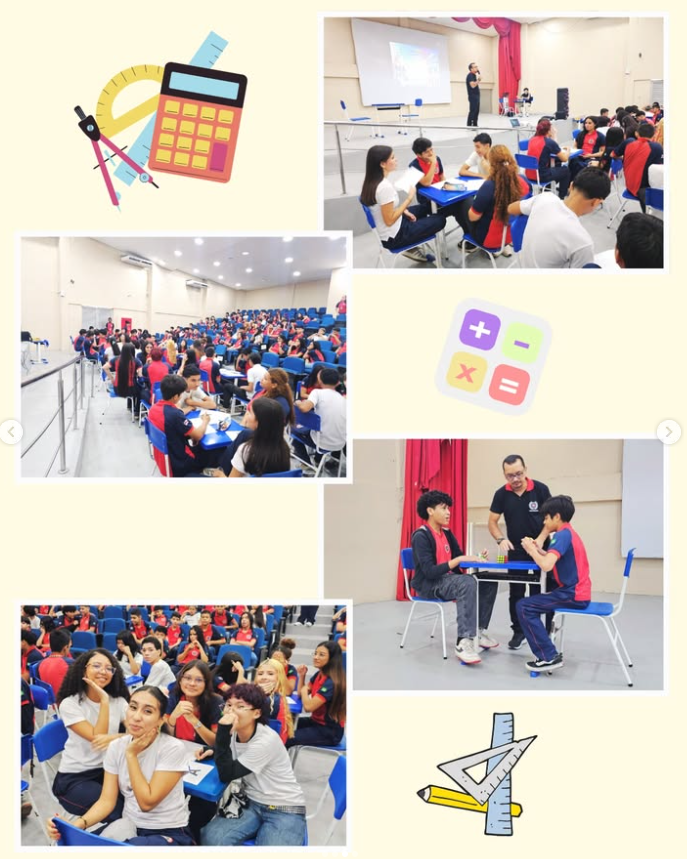
\includegraphics[scale=0.23]{imagens/gincana.png}
	\end{frame}
	
	\begin{frame}{Olimpíada Canguru de Matemática 2026}
		\centering
		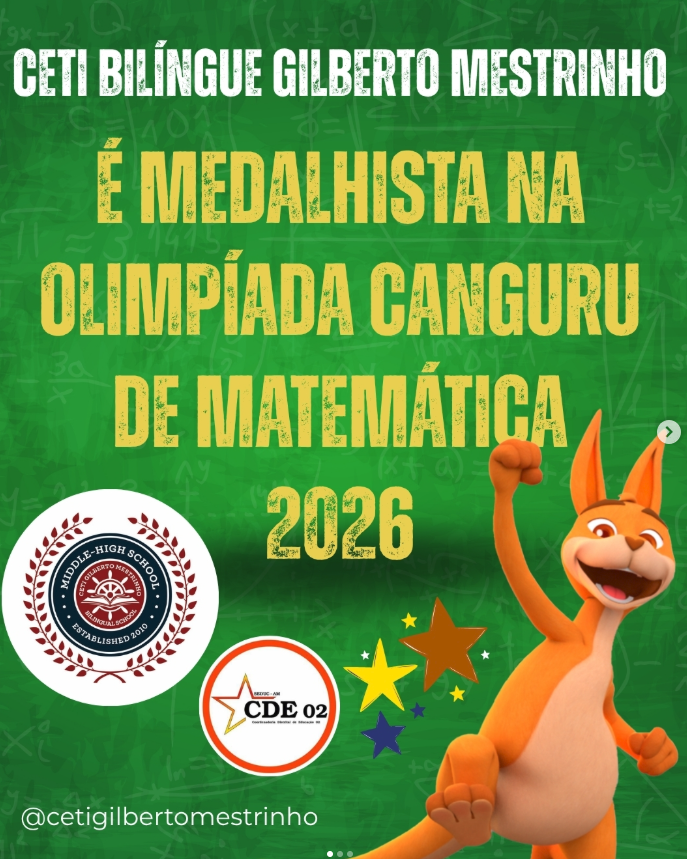
\includegraphics[scale=0.23]{imagens/canguru.png}
	\end{frame}
	
	\begin{frame}{LASERA - UEA 2026}
		\centering
		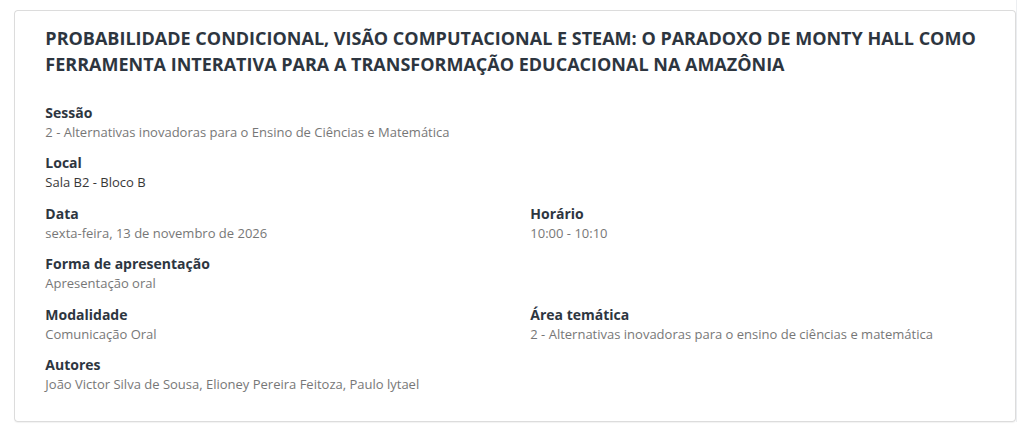
\includegraphics[scale=0.33]{imagens/lasera.png}
	\end{frame}
\section{Referência}	
	\begin{frame}{Referencial Teórico}
		\begin{itemize}
			\justifying
			\item GAMA, Larissa Tamys Barroso da. \textit{Escola Bilíngue Gilberto Mestrinho: um estudo de caso}. 2021. 63 f. Dissertação (Mestrado em Letras) -- Universidade Federal do Amazonas, Manaus, 2021.
		\end{itemize}
	\end{frame}
\end{document}